\section{Data Construction and Evaluation Population}
\label{app:data}

\subsection{Natural Sources and Paired Questions}

\dataset\ version 1.0 is a contextual composition protocol derived from the original 2WikiMultiHopQA release with entity identifiers and aliases \citep{ho2020constructing}. A source must support a unique two-edge chain whose endpoint matches the original answer. Chain eligibility requires three distinct entities, two distinct official supporting facts, and a literal object mention in the corresponding support sentence. The root and bridge subjects are matched to paragraph titles after Unicode, case, whitespace, and parenthetical-title normalization. The composed question, all ten paragraphs, and their order remain as released. The protocol adds explicit first-hop and second-hop questions while preserving each original composed task.

For seven frequent relations, constituent probes use natural templates: ``Who directed/composed $x$?'', ``Who is the father/mother/spouse of $x$?'', ``Where was $x$ born?'', and ``Where did $x$ die?'' Other relations use ``According to the evidence, for $x$, what is the value of the relation `$r$'?'' Gold aliases and demonyms are joined through the official answer entity identifier. The first-hop answer is the bridge entity; the direct second-hop and composed questions share the same endpoint aliases. These fixed diagnostic formulations make constituent correctness comparable across sources and model variants.

\cref{tab:data} describes the population. The training sources all originate in the official training split; test sources all originate in the official development split. Discovery includes 77 official training and 23 official development sources. Source identifiers are disjoint across our three splits. Forty-three test sources share a transitive root/bridge entity group with training sources. Within the test panel, all 1,000 sources have distinct roots, distinct bridges, and distinct transitive groups. Training is more concentrated in director relations (1,154/2,000 first edges) than test (280/1,000); father relations occur in 199 training and 333 test first edges.

\begin{table}[H]
  \centering
  \caption{\textbf{Source and query populations.} Every canonical source retains ten original paragraphs. A root/bridge group connects sources transitively through shared root or bridge entities. The shared-context diagnostic reuses discovery sources with a common context within each quadruplet.}
  \label{tab:data}
  \small
  \begin{tabular}{lrrrrr}
    \toprule
    \textbf{Split} & \textbf{Sources} & \textbf{Queries} & \textbf{Unique roots} & \textbf{Unique bridges} & \textbf{Entity groups} \\
    \midrule
    Discovery & 100 & 300 & 50 & 50 & 50 \\
    Training & 2,000 & 6,000 & 1,949 & 1,558 & 1,543 \\
    Test & 1,000 & 3,000 & 1,000 & 1,000 & 1,000 \\
    \midrule
    Shared-context diagnostic & 100 & 250 & \multicolumn{3}{c}{25 crossed quadruplets} \\
    \bottomrule
  \end{tabular}
\end{table}

\subsection{Fixed Source Selection}

The test panel was selected from an existing source-only pool of 1,001 examples by sorting source identifiers using a fixed SHA-256 ordering and retaining 1,000. Discovery started from 32 naturally crossed quadruplets; whole quadruplets intersecting test sources were removed, and 25 complete quadruplets were retained in a separate fixed hash ordering. Training retained 868 existing source-only examples and added 1,132 eligible official training examples, excluding selected source identifiers. Added candidates were hash-ordered and required all three prompts to fit 4,096 tokens under the original shared Qwen3 tokenizer and template. Selection uses input lengths and source annotations. The resulting source identifiers remain fixed for every model.

Eleven discovery sources use explicit official support indices: ten resolve subject/title surface mismatches, and one resolves a demonym to its answer entity. Training and test sources use the standard matching procedure. The formal splits have disjoint source identifiers; discovery and test may reuse sources from preceding development. Model-specific restoration rules were fixed during that development stage.

\subsection{Shared Contexts and Reciprocal Fact Exchanges}

Each discovery quadruplet crosses two bridges with two second-hop relations, producing four original composed questions with four distinct answer entities. We form one ten-paragraph context from complete original supporting paragraphs, padded with original non-support paragraphs from those same sources. This exact context is shared across all four composed questions and their direct probes. A quadruplet contributes four composed queries, four direct second-hop queries, and two distinct direct first-hop queries: 250 prompts and 100 three-query links in total. The construction preserves complete natural paragraphs and aligns donor and receiver evidence-token positions. These shared contexts define a separate diagnostic input from the canonical discovery contexts.

For the content intervention, we exchange the literal object spans in two official bridge facts with the same second-hop relation. The support sentence and its object span must be uniquely identifiable; the original and replacement normalized answer sets are disjoint. Exchanges preserve the question, titles, paragraph order, complete-context character multiset, and complete-context word multiset. All 100 constructed exchanges satisfy these checks and change the input. Preservation is assessed before evidence selection: rerunning a selector can subsequently produce a different retained context. This design holds the complete-context bag of words constant while changing which value is attached to the queried bridge relation. A change in the predicted value therefore measures sensitivity to the local relation binding under fixed global word counts.

\section{Experimental Protocol}
\label{app:protocol}
\subsection{Prompting, Decoding, and Answer Scoring}
\label{app:scoring_protocol}

All evaluations use native chat templates, BF16 computation, eager attention, and one-beam greedy decoding, with Qwen's optional thinking mode disabled. Each prompt contains a single user message without demonstrations. Contextual QA prompts request the answer alone in its original spelling. Question-token positions are identified from the question stem's character offsets in the native template. Batched inputs are left-padded, and responses are trimmed at the first native end-of-sequence (EOS) token.

For \dataset\ and HotpotQA, the generation budget is 32 tokens. Primary accuracy requires both EOS completion and normalized exact match against an accepted answer alias. Following the 2Wiki-MultihopQA/HotpotQA evaluator, normalization lowercases text, removes punctuation and articles, and collapses whitespace \citep{ho2020constructing,yang2018hotpotqa,alab2020twikievaluation}. We also report text exact match without the EOS condition, token F1, and completion rates (\cref{tab:scoring}). Completed-answer and text exact match coincide for the reported composed-question results.

The composition gap persists under permissive alias matching. Among the 234/236/243 failed compositions with two correct constituent answers, 14/9/6 responses contain an accepted normalized alias as a complete word sequence. Crediting these responses yields failure rates of 48.1/49.1/47.3\% on the same 457/462/501-source subsets.

For MMLU, we select the highest-probability native token among A/B/C/D at the prefill used to generate the first response token \citep{hendrycks2021mmlu}. Each label is verified to be a distinct single token. Primary accuracy is micro-averaged over all 14,042 questions; generated-letter and subject-macro accuracy provide secondary diagnostics. GSM8K prompts request step-by-step reasoning followed by a final nonempty line of the form \texttt{\#\#\#\# NUMBER} \citep{cobbe2021gsm8k}, with a generation budget of 512 tokens. After removing thousands separators, correctness is determined by decimal numerical equality. Answer validity is assessed from the final line independently of EOS, with format failures and length cutoffs recorded separately. Every method uses the same zero-shot protocol for each benchmark.

\paragraph{Text accuracy and answer completion.} \method\ increases composed text F1 from 39.48/41.87/49.83\% to 73.41/74.35/76.85\%, gains of 33.93/32.48/27.02 points. Every \method\ composed response completes within the 32-token budget. \Cref{tab:scoring} reports exact match, partial-match F1, and completion for Native, full fine-tuning, and \method.

\begin{table}[H]
  \centering
  \caption{Scoring on 1,000 composed test questions (percent; adapted methods averaged over runs). Text EM removes the EOS condition; F1 uses the same aliases.}
  \label{tab:scoring}
  \small
  \setlength{\tabcolsep}{5pt}
  % Generated by analysis/build_tables.py.
\begingroup\renewcommand{\arraystretch}{1.08}
\begin{tabular}{llrrrr}
\toprule
\textbf{Model} & \textbf{Method} & \textbf{Completed EM} & \textbf{Text EM} & \textbf{Text F1} & \textbf{EOS completion} \\
\midrule
\rowcolor{tablebase}Qwen3-4B & Native & $26.90$ & $26.90$ & $39.48$ & $96.50$ \\
 & Full fine-tuning & $57.13$ & $57.13$ & $65.26$ & $99.93$ \\
 & Evidence filtering & $47.23$ & $47.23$ & $58.66$ & $97.43$ \\
 & Head tuning & $60.13$ & $60.13$ & $67.66$ & $\mathbf{100.00}$ \\
 & Scoped adaptation & $60.43$ & $60.43$ & $67.76$ & $\mathbf{100.00}$ \\
 & Graph-first selection & $63.37$ & $63.37$ & $69.92$ & $\mathbf{100.00}$ \\
 & Attention-only reader & $\mathbf{66.80}$ & $\mathbf{66.80}$ & $\mathbf{73.43}$ & $\mathbf{100.00}$ \\
 & Metadata-only reader & $64.03$ & $64.03$ & $70.83$ & $\mathbf{100.00}$ \\
\rowcolor{tableours} & \method\ (Ours) & $\mathbf{66.80}$ & $\mathbf{66.80}$ & $73.41$ & $\mathbf{100.00}$ \\
\midrule
\rowcolor{tablebase}Qwen3-8B & Native & $29.20$ & $29.20$ & $41.87$ & $98.30$ \\
 & Full fine-tuning & $55.17$ & $55.17$ & $63.55$ & $99.93$ \\
 & Evidence filtering & $48.10$ & $48.10$ & $59.66$ & $98.10$ \\
 & Head tuning & $61.80$ & $61.80$ & $69.44$ & $\mathbf{100.00}$ \\
 & Scoped adaptation & $60.90$ & $60.90$ & $68.61$ & $\mathbf{100.00}$ \\
 & Graph-first selection & $63.70$ & $63.70$ & $70.92$ & $\mathbf{100.00}$ \\
 & Attention-only reader & $\mathbf{67.20}$ & $\mathbf{67.20}$ & $\mathbf{74.35}$ & $\mathbf{100.00}$ \\
 & Metadata-only reader & $64.60$ & $64.60$ & $71.75$ & $\mathbf{100.00}$ \\
\rowcolor{tableours} & \method\ (Ours) & $\mathbf{67.20}$ & $\mathbf{67.20}$ & $\mathbf{74.35}$ & $\mathbf{100.00}$ \\
\midrule
\rowcolor{tablebase}Llama-3.1-8B & Native & $36.40$ & $36.40$ & $49.83$ & $\mathbf{100.00}$ \\
 & Full fine-tuning & $35.20$ & $35.20$ & $44.29$ & $98.73$ \\
 & Evidence filtering & $53.43$ & $53.43$ & $64.97$ & $\mathbf{100.00}$ \\
 & Head tuning & $63.60$ & $63.60$ & $70.70$ & $\mathbf{100.00}$ \\
 & Scoped adaptation & $66.30$ & $66.30$ & $73.59$ & $\mathbf{100.00}$ \\
 & Graph-first selection & $65.73$ & $65.73$ & $72.96$ & $\mathbf{100.00}$ \\
 & Attention-only reader & $\mathbf{69.70}$ & $\mathbf{69.70}$ & $76.78$ & $\mathbf{100.00}$ \\
 & Metadata-only reader & $66.70$ & $66.70$ & $74.03$ & $\mathbf{100.00}$ \\
\rowcolor{tableours} & \method\ (Ours) & $\mathbf{69.70}$ & $\mathbf{69.70}$ & $\mathbf{76.85}$ & $\mathbf{100.00}$ \\
\bottomrule
\end{tabular}
\endgroup

\end{table}

\subsection{Selected-Head Adaptation and Fixed Restoration}
\label{app:training_protocol}

Model adaptation uses the 2,000 composed training questions. The teacher-forced objective averages cross-entropy over the gold answer and native EOS, excluding prompt tokens. We optimize zero-initialized FP32 deltas for the full-rank Q/K/V/O slices of the selected heads while freezing the base parameters. One pass through the fixed source order uses single-example microbatches, eight-example gradient accumulation, and 250 updates. AdamW \citep{loshchilov2019adamw} uses a constant learning rate of $2\times10^{-5}$, $(\beta_1,\beta_2)=(0.9,0.999)$, $\epsilon=10^{-8}$, zero weight decay, and global gradient-norm clipping at 1. The model remains in evaluation mode during adaptation, with activation checkpointing and no dropout.

\Cref{tab:parameters} reports the selected parameter counts. Projection restoration reinstates native V/O contributions at the prefill positions and layers specified in \cref{tab:scopes}, while retaining the other learned contributions. These model-specific settings were fixed before the reported evaluation suite. All component interventions share the same trained checkpoint.

\begin{table}[H]
  \centering
  \caption{Selected-head and full-reader sizes. Trainable weights count Q/K/V/O slice deltas; model fractions exclude the separately fitted reader.}
  \label{tab:parameters}
  \small
  \setlength{\tabcolsep}{5pt}
  % Generated by analysis/build_tables.py.
\begin{tabular}{lrrrr}
\toprule
Model & Selected heads & Reader weights & Trainable weights & Model fraction \\
\midrule
Qwen3-4B & 20 & 42 & 23,592,960 & 0.587\% \\
Qwen3-8B & 20 & 42 & 39,845,888 & 0.486\% \\
Llama-3.1-8B & 40 & 82 & 75,497,472 & 0.940\% \\
\bottomrule
\end{tabular}

\end{table}

\begin{table}[H]
  \centering
  \caption{Fixed native-projection restoration rules, with zero-based layer indices. Restoration affects selected-head contributions at the specified prefill positions.}
  \label{tab:scopes}
  \small
  \setlength{\tabcolsep}{6pt}
  \begin{tabular}{llll}
    \toprule
    \textbf{Model} & \textbf{Projections restored} & \textbf{Layers} & \textbf{Token positions} \\
    \midrule
    Qwen3-4B & V and O & 16--19 & Prefix before the question \\
    Qwen3-8B & V and O & 12--19 & Question prefill \\
    Llama-3.1-8B & V & All selected layers & Prefix before the question \\
    \bottomrule
  \end{tabular}
\end{table}

\subsection{Fitting and Applying the Paragraph-Address Readout}
\label{app:readout_protocol}

Each selected head contributes two paragraph features: the logarithm of the mean question-token attention mass and the logarithm of the mass at the final question token. Masses are floored at $10^{-8}$ before taking logarithms. Two metadata features encode the log paragraph-to-prompt token ratio and whether the paragraph title appears in the question. The title feature uses normalized substring matching for Qwen and normalized whole-word matching for Llama; candidate graphs use whole-word matching for both families. Full readers contain 42/42/82 weights. Attention-only readers use the head features, while metadata-only readers use the two metadata features.

Standardization and fitting use the 2,000 composed training examples. Features are standardized across all training paragraphs, with population standard deviations floored at $10^{-4}$. The zero-initialized linear scorer is optimized for 500 full-batch Adam steps \citep{kingma2015adam}, using learning rate 0.03 and penalty $0.01\lVert w\rVert_2^2$. The cross-entropy objective identifies the annotated bridge among the original paragraphs. We omit a shared intercept because it cancels in the paragraph-wise softmax. Native and adapted models each receive a separately fitted, state-aligned reader. At inference, the frozen scorer resolves ambiguous candidates derived from the input. Unique candidates require no attention prefill, and inapplicable graphs retain the original context.

\subsection{Full-Parameter Comparison and Training Cost}
\label{app:fullft_protocol}

Full fine-tuning updates all model parameters in training mode, using the same objective, source count, gradient accumulation, learning rate, and optimizer hyperparameters. It uses BF16 weights, CPU-offloaded FP32 optimizer state, and seed-dependent source permutations. This recipe is shared across all three models, and both training methods perform 250 updates. Under the recorded shared-resource schedule, head adaptation averages 552/1,566/747 seconds, compared with 4,007/34,916/41,512 seconds for full fine-tuning (\cref{tab:training_cost}). Answer-format and completion rates are reported in \cref{tab:secondary_qa}.

\begin{table}[H]
  \centering
  \caption{Training workload and measured duration across three recorded runs. Both methods use one pass over 2,000 composed sources.}
  \label{tab:training_cost}
  \small
  \setlength{\tabcolsep}{5pt}
  % Generated by analysis/build_tables.py.
\begingroup\renewcommand{\arraystretch}{1.08}
\begin{tabular}{llrrrr}
\toprule
\textbf{Model} & \textbf{Training} & \textbf{Sources} & \textbf{Updates} & \textbf{Weights (M)} & \textbf{Seconds, mean (range)} \\
\midrule
Qwen3-4B & Full fine-tuning & 2000 & 250 & 4022.47 & 4007 (3970--4031) \\
\rowcolor{tableours} & \method\ adaptation (Ours) & 2000 & 250 & 23.59 & 552 (496--656) \\
\midrule
Qwen3-8B & Full fine-tuning & 2000 & 250 & 8190.74 & 34916 (32817--37643) \\
\rowcolor{tableours} & \method\ adaptation (Ours) & 2000 & 250 & 39.85 & 1566 (1361--1787) \\
\midrule
Llama-3.1-8B & Full fine-tuning & 2000 & 250 & 8030.26 & 41512 (29470--47703) \\
\rowcolor{tableours} & \method\ adaptation (Ours) & 2000 & 250 & 75.50 & 747 (722--768) \\
\bottomrule
\end{tabular}
\endgroup

\end{table}

\subsection{Recorded Runs and Statistical Uncertainty}
\label{app:uncertainty}

The three recorded runs use seed identifiers 42/43/44. With fixed source order, zero initialization, and evaluation mode, selected-head adaptation produces identical loss and gradient-norm sequences across runs; reader fitting is also deterministic. Reported sample standard deviations summarize variation across the recorded evaluations, whose individual composed scores appear in \cref{tab:per_run}.

For native and selected-head contextual QA evaluations, Qwen3-4B and Llama use batch size 1 in run 42 and 4 in runs 43/44; Qwen3-8B uses 4 throughout. MMLU also uses batch size 4 throughout. GSM8K uses 1/1/4 for Qwen3-4B, 4/4/4 for Qwen3-8B, and 1/1/1 for Llama. Full-parameter evaluations all use batch size 4. BF16 greedy decoding can produce small batch-dependent differences. Qwen3-8B's main native composed accuracy is 29.2\%, compared with 28.9\% in its batch-1 access and necessity experiments. Each causal contrast is paired with the native reference from the same experiment.

Confidence intervals in \cref{tab:paired_effects} use paired percentile bootstraps with 2,000 replicates and random seed 42. For repair comparisons, we average each source's correctness over the three runs and then resample source groups defined by transitively shared normalized root/bridge titles. Each of the 1,000 test groups contains one source. The resulting intervals quantify source-sampling variation on the fixed panel. Factorial contrasts instead resample the 25 shared-context quadruplets, preserving all four receivers and their paired intervention arms within each group.

\begin{table}[H]
  \centering
  \caption{Paired composed-accuracy changes in percentage points, with 95\% bootstrap intervals. Repair comparisons use source-wise run averages; bridge calibration uses its own experiment's native reference.}
  \label{tab:paired_effects}
  \small
  \setlength{\tabcolsep}{5pt}
  % Generated by analysis/build_tables.py.
\begingroup\renewcommand{\arraystretch}{1.08}
\begin{tabular}{lrrr}
\toprule
\textbf{Paired contrast} & \textbf{Qwen3-4B} & \textbf{Qwen3-8B} & \textbf{Llama-3.1-8B} \\
\midrule
\method\ $-$ Native & $39.90\;[36.73, 43.03]$ & $38.00\;[34.70, 41.40]$ & $33.30\;[30.23, 36.50]$ \\
Full readout $-$ paragraph order & $3.43\;[2.40, 4.63]$ & $3.50\;[2.40, 4.80]$ & $3.97\;[2.87, 5.30]$ \\
Bridge calibration $-$ Native & $4.90\;[2.90, 6.80]$ & $5.50\;[3.70, 7.40]$ & $16.00\;[13.40, 18.60]$ \\
\bottomrule
\end{tabular}
\endgroup

\end{table}

\begin{table}[H]
  \centering
  \caption{Composed accuracy (percent) on the same 1,000 test sources for each recorded run. Interpretation of run dispersion follows Appendix~\ref{app:uncertainty}.}
  \label{tab:per_run}
  \small
  \setlength{\tabcolsep}{6pt}
  % Generated by analysis/build_tables.py.
\begingroup\renewcommand{\arraystretch}{1.08}
\begin{tabular}{llrrr}
\toprule
\textbf{Model} & \textbf{Method} & \textbf{Run 42} & \textbf{Run 43} & \textbf{Run 44} \\
\midrule
Qwen3-4B & Full fine-tuning & 54.4 & 58.6 & 58.4 \\
\rowcolor{tableours} & \method\ (Ours) & 66.4 & 67.0 & 67.0 \\
\midrule
Qwen3-8B & Full fine-tuning & 52.7 & 61.3 & 51.5 \\
\rowcolor{tableours} & \method\ (Ours) & 67.2 & 67.2 & 67.2 \\
\midrule
Llama-3.1-8B & Full fine-tuning & 32.8 & 33.7 & 39.1 \\
\rowcolor{tableours} & \method\ (Ours) & 69.5 & 69.8 & 69.8 \\
\bottomrule
\end{tabular}
\endgroup

\end{table}


\section{Localization and Factorized Interventions}
\label{app:interventions}

\subsection{Head Ranking and Count Selection}

The ranking in \cref{eq:ranking} uses discovery-only paired direct-target and composed queries under their original contexts. \cref{fig:localization} plots the complete layer/head score maps and marks selected heads. The ranking measures the access contribution of each head under the paired queries. For each candidate count, the calibration intervention sets bridge mass using discovery-derived, head-specific targets; \cref{tab:head_selection} reports the composed accuracies used to choose 20, 20, and 40 heads. A tie favors the smaller set. The shared-context factorial experiment uses these frozen choices.

\begin{figure}[H]
  \centering
  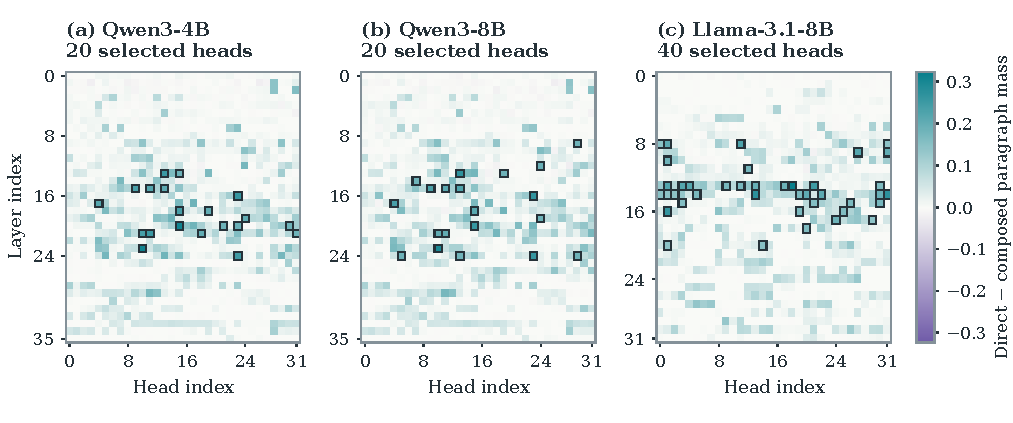
\includegraphics[width=\textwidth]{figures/data_app_localization.pdf}
  \caption{\textbf{Complete head-localization maps.} Color denotes the discovery mean difference in bridge-paragraph attention between the direct second-hop and composed questions, averaged over question-token rows. Marked cells identify the selected head set for each model. Layer and head indices are zero-based. The maps reveal the distribution of query-dependent evidence access across the model.}
  \label{fig:localization}
\end{figure}

\begin{table}[H]
  \centering
  \caption{\textbf{Discovery-only head-count selection.} Composed accuracy (\%) on 100 canonical discovery sources under annotated bridge-mass calibration. Bold marks the selected count; ties favor fewer heads. These native scores differ from the shared-context diagnostic because the supplied contexts differ.}
  \label{tab:head_selection}
  \small
  \begin{tabular}{lrrrr}
    \toprule
    \textbf{Model} & \textbf{Native} & \textbf{Top 20} & \textbf{Top 40} & \textbf{Top 80} \\
    \midrule
    Qwen3-4B & 35 & \cellcolor{tableours}\textbf{36} & 36 & 33 \\
    Qwen3-8B & 45 & \cellcolor{tableours}\textbf{47} & 47 & 45 \\
    Llama-3.1-8B & 45 & 64 & \cellcolor{tableours}\textbf{66} & 58 \\
    \bottomrule
  \end{tabular}
\end{table}

\subsection{Head Necessity and Address Controls}

For head knockout, selected head outputs are set to zero before their output projection at all question-prefill positions. Prefix computation and cached decoding retain their ordinary forward operations. We compare the top 20, 40, and 80 heads to one layer-matched random set at each count, sampled with seeds 62, 82, and 122, respectively. Random sets preserve the number of selected heads in each layer and may overlap the ranked set. The overlap counts at these three doses are 3/7/13 for Qwen3-4B, 0/4/15 for Qwen3-8B, and 3/8/21 for Llama.

\cref{fig:necessity} reports all three query types and all doses on the 1,000-source test panel. At the chosen counts, selected knockout reduces composed accuracy to 7.4/5.5/6.4\%, compared with 24.4/27.3/29.4\% for matched random knockout. The substantial constituent effects show that these heads contribute causally across query types. For paragraph-address controls, the same frozen targets are applied either to the annotated bridge, the root, or the other paragraph with nearest token length (ties are broken by title and then original index). The paired differences in \cref{fig:causal} use each intervention pipeline's own native baseline.

\begin{figure}[H]
  \centering
  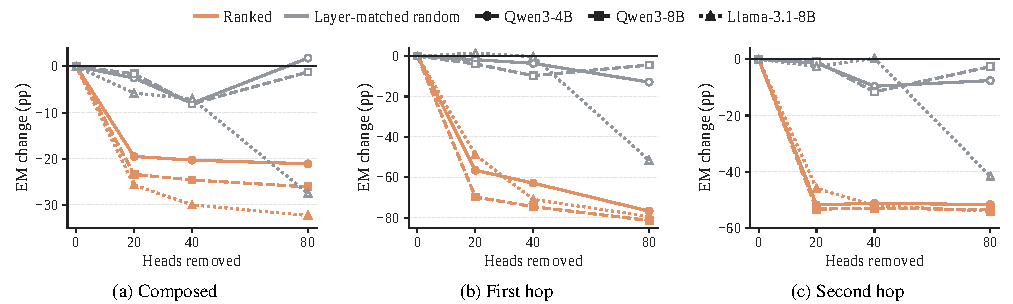
\includegraphics[width=\textwidth]{figures/data_app_necessity.pdf}
  \caption{\textbf{Necessity across query types and knockout doses.} Completed-answer EM on 1,000 test sources, with models in columns and composed, direct first-hop, and direct second-hop questions in rows. Ranked-head knockout is compared with layer-matched random-head knockout at counts 20, 40, and 80. Zero denotes the native model in this pipeline. Each random point uses one matched set; lines connect measured doses. Vertical dotted guides mark the chosen head counts of 20/20/40.}
  \label{fig:necessity}
\end{figure}

\subsection{Exact Attention Transformations}

Consider a selected head and a question-token row $a_k$, with bridge key positions $B$, total mass $T=\sum_k a_k$, and bridge mass $m=\sum_{k\in B}a_k$. Let $\tau\in[0,1]$ be its frozen target fraction. In exact arithmetic $T=1$; retaining the measured $T$ avoids attributing floating-point row-sum differences to the intervention. Mass calibration is
\begin{equation}
 a'_k=\begin{cases}
 \tau T\,a_k/m, & k\in B,\\
 (1-\tau)T\,a_k/(T-m), & k\notin B.
 \end{cases}
 \label{eq:mass_appendix}
\end{equation}
The donor conditional $\rho_k^{\mathrm{dir}}$ is obtained by normalizing bridge attention at the final token of the paired direct second-hop question. Pattern-only transfer sets $a'_k=m\rho_k^{\mathrm{dir}}$ inside $B$ and retains the outside allocation; the combined intervention sets $a'_k=\tau T\rho_k^{\mathrm{dir}}$ inside $B$ and uses the second line of \cref{eq:mass_appendix} outside. The same donor conditional is applied to every receiver question-token row. Operations are evaluated in FP32 and cast once to the native attention dtype. Rows with nonfinite or negative values, zero source or outside mass, or invalid donor probabilities retain their original distribution.

Donor and receiver must have identical context-token prefixes and bridge-key positions. We transfer only normalized attention distributions; the receiving run computes its own value vectors and output projections. As with activation interventions more broadly \citep{meng2022locating,zhang2024patching}, the changed attention can propagate through downstream activations. Subsequent cache states follow the resulting forward pass. The identity condition bypasses replacement and reproduces native generated token identifiers exactly for all 300 model/source combinations.

\cref{tab:factorial} gives all paired factorial contrasts. The pattern effect changes from $-6/+2/-4$ points at native mass to $+2/+7/+12$ points at calibrated mass. The interaction estimates are $+8$, $+5$, and $+16$ points, with 95\% intervals $[1,14]$, $[0,10]$, and $[8,25]$. Mass calibration increases accuracy by 15/9/29 points with the direct-query pattern, compared with 7/4/13 points under the receiver pattern. Thus, the crossed interventions show that access allocation and local reading reinforce one another.

\begin{table}[H]
  \centering
  \caption{\textbf{Factorial effects on shared-context composition.} Accuracy differences in percentage points with 95\% paired percentile intervals from 2,000 resamples of the 25 quadruplets. All 100 composed receivers remain in every condition. The interaction is defined in \cref{eq:interaction}; Qwen3-8B's interval includes zero at its boundary.}
  \label{tab:factorial}
  \small\setlength{\tabcolsep}{4pt}
  % Generated by analysis/build_tables.py.
\begingroup\renewcommand{\arraystretch}{1.08}
\begin{tabular}{lrrr}
\toprule
\textbf{Contrast} & \textbf{Qwen3-4B} & \textbf{Qwen3-8B} & \textbf{Llama-3.1-8B} \\
\midrule
Mass effect, receiver pattern & $+7.0\;[+1.0, +14.0]$ & $+4.0\;[-1.0, +10.0]$ & $+13.0\;[+6.0, +20.0]$ \\
Mass effect, direct-query pattern & $+15.0\;[+9.0, +22.0]$ & $+9.0\;[+4.0, +14.0]$ & $+29.0\;[+20.0, +38.0]$ \\
Pattern effect, native mass & $-6.0\;[-10.0, -2.0]$ & $+2.0\;[-3.0, +7.0]$ & $-4.0\;[-9.0, +1.0]$ \\
Pattern effect, calibrated mass & $+2.0\;[-3.0, +7.0]$ & $+7.0\;[+3.0, +11.0]$ & $+12.0\;[+3.0, +21.0]$ \\
\rowcolor{tableours}Mass $\times$ pattern interaction & $+8.0\;[+1.0, +14.0]$ & $+5.0\;[+0.0, +10.0]$ & $+16.0\;[+8.0, +25.0]$ \\
\bottomrule
\end{tabular}
\endgroup

\end{table}

\subsection{Readout and Content Diagnostics}

\cref{tab:readouts} reports the full, attention-only, and metadata-only readouts both across all test sources and within native constituent-correct composition failures. Native and scoped readouts are fitted separately on features from their respective model states. The full readout improves from 80.3/83.9/91.9\% in the native state to 90.3/92.6/95.0\% in the adapted state. On native composition failures, accuracy rises from 72.2/74.6/86.0\% to 82.9/86.0/92.2\%. Attention-only readouts show the same improvement, reaching 89.6/91.2/94.3\% overall. Metadata accuracy stays at 43.5/43.5/44.1\%, so the improvement comes from the adapted attention features.

\begin{table}[H]
  \centering
  \caption{\textbf{Paragraph-address readout diagnostics.} Accuracy (\%) of training-fitted readouts. ``Failure subset'' is fixed by the native model: both constituents are correct and the composition is wrong. Native-state rows distinguish attention information from paragraph-length/title cues; scoped-state rows use the deployed model's own features. A common intercept would cancel in the paragraph softmax, so each readout has no bias parameter.}
  \label{tab:readouts}
  \small\setlength{\tabcolsep}{6pt}
  % Generated by analysis/build_tables.py.
\begin{tabular}{llrrrrrr}
\toprule
 &  & \multicolumn{3}{c}{All test sources ($n=1{,}000$)} & \multicolumn{3}{c}{Native composition failures} \\
\cmidrule(lr){3-5}\cmidrule(lr){6-8}
Model & Model state & Full & Attention & Metadata & Full & Attention & Metadata \\
\midrule
Qwen3-4B & Native & 80.3 & 75.0 & 43.5 & 72.2 & 64.5 & 39.7 \\
 & Scoped adaptation & 90.3 & 89.6 & 43.5 & 82.9 & 80.3 & 39.7 \\
\midrule
Qwen3-8B & Native & 83.9 & 79.3 & 43.5 & 74.6 & 70.3 & 42.4 \\
 & Scoped adaptation & 92.6 & 91.2 & 43.5 & 86.0 & 82.2 & 42.4 \\
\midrule
Llama-3.1-8B & Native & 91.9 & 90.9 & 44.1 & 86.0 & 84.4 & 42.8 \\
 & Scoped adaptation & 95.0 & 94.3 & 44.1 & 92.2 & 90.9 & 42.8 \\
\bottomrule
\end{tabular}

\end{table}

\cref{tab:content} provides all content-exchange outcomes. Edited-value following and obsolete-answer persistence are measured against disjoint alias sets; joint accuracy additionally requires that the same source be answered correctly before the exchange. The joint measure captures correct answers in both versions of the same example. All displayed content metrics agree across the three recorded runs. Annotated bridge-mass calibration increases following by 9/2/20 points over Native. The complete repair increases following by 51/41/48 points and joint accuracy by 54/43/48 points. Relative to scoped adaptation, it reduces obsolete-answer persistence from 17/23/16\% to 9/7/4\%, linking evidence selection to more consistent updates.

\begin{table}[H]
  \centering
  \caption{\textbf{Complete reciprocal content-exchange outcomes.} Accuracy (\%) on 100 composed queries from 25 shared-context quadruplets. Original accuracy uses the original answer, following uses the exchanged value, persistence uses the now-obsolete answer, and joint accuracy requires correctness before and after exchange. Values are mean $\pm$ sample SD across recorded runs; all SDs here are zero. Every example undergoes a valid reciprocal exchange.}
  \label{tab:content}
  \small\setlength{\tabcolsep}{5pt}
  % Generated by analysis/build_tables.py.
\begingroup\renewcommand{\arraystretch}{1.08}
\begin{tabular}{llrrrr}
\toprule
\textbf{Model} & \textbf{Method} & \textbf{Original EM $\uparrow$} & \textbf{Edited-value EM $\uparrow$} & \textbf{Old persistence $\downarrow$} & \textbf{Joint EM $\uparrow$} \\
\midrule
\rowcolor{tablebase}Qwen3-4B & Native & $34.0$ & $26.0$ & $\mathbf{8.0}$ & $21.0$ \\
 & Mass calibration & $41.0$ & $35.0$ & $\mathbf{8.0}$ & $29.0$ \\
 & Scoped adaptation & $77.0{\color{black!60}\,\pm\,0.0}$ & $64.0{\color{black!60}\,\pm\,0.0}$ & $17.0{\color{black!60}\,\pm\,0.0}$ & $57.0{\color{black!60}\,\pm\,0.0}$ \\
\rowcolor{tableours} & \method\ (Ours) & $\mathbf{88.0}{\color{black!60}\,\pm\,0.0}$ & $\mathbf{77.0}{\color{black!60}\,\pm\,0.0}$ & $9.0{\color{black!60}\,\pm\,0.0}$ & $\mathbf{75.0}{\color{black!60}\,\pm\,0.0}$ \\
\midrule
\rowcolor{tablebase}Qwen3-8B & Native & $48.0$ & $35.0$ & $11.0$ & $29.0$ \\
 & Mass calibration & $52.0$ & $37.0$ & $12.0$ & $31.0$ \\
 & Scoped adaptation & $82.0{\color{black!60}\,\pm\,0.0}$ & $66.0{\color{black!60}\,\pm\,0.0}$ & $23.0{\color{black!60}\,\pm\,0.0}$ & $60.0{\color{black!60}\,\pm\,0.0}$ \\
\rowcolor{tableours} & \method\ (Ours) & $\mathbf{84.0}{\color{black!60}\,\pm\,0.0}$ & $\mathbf{76.0}{\color{black!60}\,\pm\,0.0}$ & $\mathbf{7.0}{\color{black!60}\,\pm\,0.0}$ & $\mathbf{72.0}{\color{black!60}\,\pm\,0.0}$ \\
\midrule
\rowcolor{tablebase}Llama-3.1-8B & Native & $51.0$ & $32.0$ & $14.0$ & $29.0$ \\
 & Mass calibration & $64.0$ & $52.0$ & $9.0$ & $49.0$ \\
 & Scoped adaptation & $85.0{\color{black!60}\,\pm\,0.0}$ & $72.0{\color{black!60}\,\pm\,0.0}$ & $16.0{\color{black!60}\,\pm\,0.0}$ & $69.0{\color{black!60}\,\pm\,0.0}$ \\
\rowcolor{tableours} & \method\ (Ours) & $\mathbf{88.0}{\color{black!60}\,\pm\,0.0}$ & $\mathbf{80.0}{\color{black!60}\,\pm\,0.0}$ & $\mathbf{4.0}{\color{black!60}\,\pm\,0.0}$ & $\mathbf{77.0}{\color{black!60}\,\pm\,0.0}$ \\
\bottomrule
\end{tabular}
\endgroup

\end{table}

\section{Evidence Selection and Complete Application Results}
\label{app:application}

\subsection{Input-Derived Candidates and Ambiguous Cases}

Titles and question text are Unicode-normalized, case-folded, and split into word sequences. A title is matched as a whole normalized word sequence. Nested title matches are removed, and independently mentioned entities retain separate matches. The graph applies only when the question has exactly one distinct maximally matched title. Its outgoing candidates are other paragraph titles appearing in that root paragraph's body, in original paragraph order. Question text, paragraph titles, and paragraph bodies supply all graph inputs.

On the 1,000 composed test questions, there are 75 inapplicable/no-candidate cases, 822 unique-candidate cases, and 103 ambiguous cases. The latter comprise 86 two-candidate, 16 three-candidate, and one four-candidate case. The annotated bridge appears among candidates for 918 questions; the unique candidate is correct in 817/822 cases. Unique candidates are selected without a readout pass. For ambiguity, the full-context composed prefill supplies attention features, and the maximum-scoring candidate is selected. The retained root and candidate paragraphs preserve their original order. Inapplicable inputs preserve their complete context.

\cref{tab:ambiguity} isolates the 103 ambiguous cases. The graph-first policy chooses the first outgoing candidate, while the readout policies change only this choice under the same scoped model. Full-reader bridge selection succeeds on 95/96/98 cases, compared with 37 for graph-first. Attention-only selection succeeds on 94/97/97, and metadata-only on 57/57/59. Full and attention-only readouts yield the same composed EM on the full panel, with some differences in bridge choices and individual answers. Their shared aggregate gain shows that the attention features suffice for effective disambiguation. Relative to scoped adaptation on these ambiguous questions, the full repair adds 10.4/5.8/3.6 points of composed accuracy.

\begin{table}[H]
  \centering
  \caption{\textbf{Where the attention readout changes evidence selection.} Results on the 103 composed questions whose input-derived graph has multiple candidates. Every policy uses the same scoped model and retains the root plus one candidate paragraph. Bridge accuracy is evaluated against annotations only after selection. Values are percentages, mean $\pm$ sample SD. The full repair and graph-first produce identical generated token sequences on all other 897 questions in every recorded run.}
  \label{tab:ambiguity}
  \small\setlength{\tabcolsep}{8pt}
  % Generated by analysis/build_tables.py.
\begingroup\renewcommand{\arraystretch}{1.08}
\begin{tabular}{llrr}
\toprule
\textbf{Model} & \textbf{Candidate ranking} & \textbf{Bridge address $\uparrow$} & \textbf{Composed EM $\uparrow$} \\
\midrule
\rowcolor{tablebase}Qwen3-4B & Paragraph order & $35.9$ & $36.9{\color{black!80}\,\pm\,0.0}$ \\
 & Metadata features & $55.3$ & $43.4{\color{black!80}\,\pm\,0.6}$ \\
 & Attention features & $91.3$ & $\mathbf{70.2}{\color{black!80}\,\pm\,1.1}$ \\
\rowcolor{tableours} & Full features & $\mathbf{92.2}$ & $\mathbf{70.2}{\color{black!80}\,\pm\,1.1}$ \\
\midrule
\rowcolor{tablebase}Qwen3-8B & Paragraph order & $35.9$ & $36.9{\color{black!80}\,\pm\,0.0}$ \\
 & Metadata features & $55.3$ & $45.6{\color{black!80}\,\pm\,0.0}$ \\
 & Attention features & $\mathbf{94.2}$ & $\mathbf{70.9}{\color{black!80}\,\pm\,0.0}$ \\
\rowcolor{tableours} & Full features & $93.2$ & $\mathbf{70.9}{\color{black!80}\,\pm\,0.0}$ \\
\midrule
\rowcolor{tablebase}Llama-3.1-8B & Paragraph order & $35.9$ & $38.2{\color{black!80}\,\pm\,0.6}$ \\
 & Metadata features & $57.3$ & $47.6{\color{black!80}\,\pm\,0.0}$ \\
 & Attention features & $94.2$ & $\mathbf{76.7}{\color{black!80}\,\pm\,0.0}$ \\
\rowcolor{tableours} & Full features & $\mathbf{95.1}$ & $\mathbf{76.7}{\color{black!80}\,\pm\,0.0}$ \\
\bottomrule
\end{tabular}
\endgroup

\end{table}

\subsection{All Constituents and Component Ablations}

\cref{tab:core_complete} reports all three query types and their joint accuracy for every variant. \cref{fig:ablations} compares the component variants on composed accuracy. The native-evidence-filtering variant uses a native-state reader and the native model; all variants built from selected-head adaptation share its checkpoint. The scoped variant changes the fixed restoration rule; graph-first, full-reader, attention-only, and metadata-only variants then use that same scoped model. This organization distinguishes gains from adapting answer computation, selecting paragraphs, and resolving candidate ambiguity.

\paragraph{Constituent and joint improvements.} Evidence filtering alone improves composed accuracy by 20.3/18.9/17.0 points and all-three accuracy by 10.8/11.2/13.7 points over Native. Selected-head tuning improves second-hop accuracy by 14.2/15.7/9.9 points. Adding fixed restoration improves first-hop accuracy over head tuning by 5.0/2.4/27.3 points and all-three accuracy by 2.4/0.8/17.5 points. The complete repair reaches 41.3/45.4/42.3\% all-three accuracy, compared with 22.3/22.6/25.8\% natively. The highest all-three scores are 41.8\% for Qwen3-4B and 42.5\% for Llama under scoped adaptation, and 45.4\% for Qwen3-8B under the complete repair. Complete first-hop, second-hop, and composed scores appear together in \cref{tab:core_complete}.

\begin{table}[H]
  \centering
  \caption{\textbf{Complete contextual reasoning results.} Completed-answer EM (\%) on all 1,000 sources per query type. ``All three'' requires a source's composed, first-hop, and second-hop answers to be correct. Values are mean $\pm$ sample SD over three recorded runs; Native is measured once. The displayed dispersion follows the conventions in \cref{app:uncertainty}.}
  \label{tab:core_complete}
  \small\setlength{\tabcolsep}{4pt}
  % Generated by analysis/build_tables.py.
\begin{tabular}{llrrrr}
\toprule
Model & Method & Composed & First hop & Target hop & All three \\
\midrule
Qwen3-4B & Native & $26.90$ & $87.20$ & $52.90$ & $22.30$ \\
 & Evidence filtering & $47.23\,\pm\,0.12$ & $88.33\,\pm\,0.12$ & $52.93\,\pm\,0.06$ & $33.13\,\pm\,0.06$ \\
 & Head tuning & $60.13\,\pm\,0.12$ & $66.27\,\pm\,0.12$ & $67.13\,\pm\,0.06$ & $39.40\,\pm\,0.00$ \\
 & Scoped adaptation & $60.43\,\pm\,0.12$ & $71.27\,\pm\,0.29$ & $67.63\,\pm\,0.06$ & $41.80\,\pm\,0.00$ \\
 & Graph-first selection & $63.37\,\pm\,0.23$ & $70.40\,\pm\,0.00$ & $67.57\,\pm\,0.12$ & $39.23\,\pm\,0.06$ \\
 & \method & $66.80\,\pm\,0.35$ & $69.80\,\pm\,0.00$ & $67.57\,\pm\,0.12$ & $41.33\,\pm\,0.06$ \\
 & Attention-only reader & $66.80\,\pm\,0.35$ & $69.80\,\pm\,0.00$ & $67.57\,\pm\,0.12$ & $41.43\,\pm\,0.06$ \\
 & Metadata-only reader & $64.03\,\pm\,0.29$ & $70.40\,\pm\,0.00$ & $67.57\,\pm\,0.12$ & $39.90\,\pm\,0.00$ \\
 & Full fine-tuning & $57.13\,\pm\,2.37$ & $29.97\,\pm\,4.52$ & $58.90\,\pm\,2.51$ & $17.40\,\pm\,2.16$ \\
\midrule
Qwen3-8B & Native & $29.20$ & $86.00$ & $54.40$ & $22.60$ \\
 & Evidence filtering & $48.10\,\pm\,0.00$ & $89.10\,\pm\,0.00$ & $54.90\,\pm\,0.00$ & $33.80\,\pm\,0.00$ \\
 & Head tuning & $61.80\,\pm\,0.00$ & $70.20\,\pm\,0.00$ & $70.10\,\pm\,0.00$ & $41.60\,\pm\,0.00$ \\
 & Scoped adaptation & $60.90\,\pm\,0.00$ & $72.60\,\pm\,0.00$ & $70.40\,\pm\,0.00$ & $42.40\,\pm\,0.00$ \\
 & Graph-first selection & $63.70\,\pm\,0.00$ & $73.40\,\pm\,0.00$ & $70.10\,\pm\,0.00$ & $43.30\,\pm\,0.00$ \\
 & \method & $67.20\,\pm\,0.00$ & $73.40\,\pm\,0.00$ & $70.10\,\pm\,0.00$ & $45.40\,\pm\,0.00$ \\
 & Attention-only reader & $67.20\,\pm\,0.00$ & $73.40\,\pm\,0.00$ & $70.10\,\pm\,0.00$ & $45.40\,\pm\,0.00$ \\
 & Metadata-only reader & $64.60\,\pm\,0.00$ & $73.80\,\pm\,0.00$ & $70.10\,\pm\,0.00$ & $44.10\,\pm\,0.00$ \\
 & Full fine-tuning & $55.17\,\pm\,5.35$ & $28.47\,\pm\,8.81$ & $56.93\,\pm\,5.42$ & $14.13\,\pm\,5.84$ \\
\midrule
Llama-3.1-8B & Native & $36.40$ & $85.20$ & $58.60$ & $25.80$ \\
 & Evidence filtering & $53.43\,\pm\,0.06$ & $85.07\,\pm\,0.12$ & $58.70\,\pm\,0.00$ & $39.53\,\pm\,0.12$ \\
 & Head tuning & $63.60\,\pm\,0.17$ & $37.57\,\pm\,0.12$ & $68.50\,\pm\,0.00$ & $24.97\,\pm\,0.12$ \\
 & Scoped adaptation & $66.30\,\pm\,0.00$ & $64.87\,\pm\,0.12$ & $70.80\,\pm\,0.00$ & $42.50\,\pm\,0.17$ \\
 & Graph-first selection & $65.73\,\pm\,0.12$ & $66.60\,\pm\,0.17$ & $70.20\,\pm\,0.00$ & $40.40\,\pm\,0.00$ \\
 & \method & $69.70\,\pm\,0.17$ & $65.97\,\pm\,0.12$ & $70.20\,\pm\,0.00$ & $42.30\,\pm\,0.00$ \\
 & Attention-only reader & $69.70\,\pm\,0.17$ & $65.97\,\pm\,0.12$ & $70.20\,\pm\,0.00$ & $42.30\,\pm\,0.00$ \\
 & Metadata-only reader & $66.70\,\pm\,0.17$ & $66.80\,\pm\,0.17$ & $70.20\,\pm\,0.00$ & $41.10\,\pm\,0.00$ \\
 & Full fine-tuning & $35.20\,\pm\,3.41$ & $12.13\,\pm\,3.00$ & $33.50\,\pm\,4.45$ & $3.60\,\pm\,0.70$ \\
\bottomrule
\end{tabular}

\end{table}

\begin{figure}[H]
  \centering
  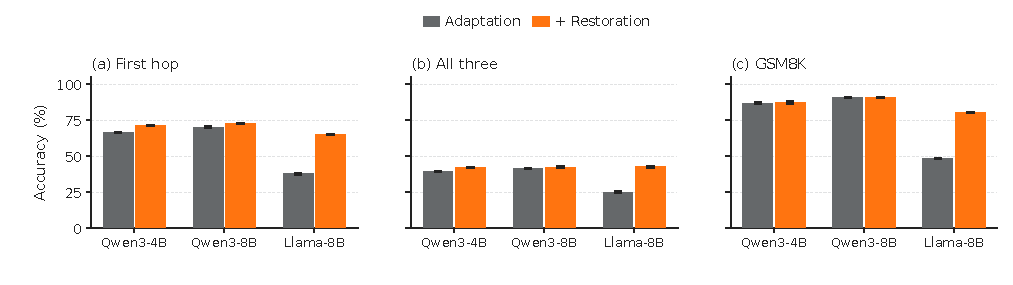
\includegraphics[width=\textwidth]{figures/data_app_ablation.pdf}
  \caption{\textbf{Component ablations on composed questions.} Completed-answer accuracy on 1,000 test sources. Points summarize recorded-run means and error bars show sample SD under the conventions of \cref{app:uncertainty}. Attention-only and full readouts coincide on composed accuracy, while metadata-only selection is weaker. Complete constituent and joint outcomes appear in \cref{tab:core_complete}.}
  \label{fig:ablations}
\end{figure}

\paragraph{Composition within each model's correct-constituent set.} \Cref{tab:conditional_composition} applies \cref{eq:cfr} to every model variant. \method\ reduces the conditional composition failure rate from 51.2/51.1/48.5\% to 11.6/10.8/8.6\%. Each row uses that variant's own set of correctly answered constituent pairs; the table reports both the population size and number of failed compositions. The fixed-native-population analysis below follows the original failures and successes across variants.

\begin{table}[H]
  \centering
  \caption{\textbf{Conditional composition failure across model variants.} Every method answers all 1,000 triplets. The constituent-correct count is the number of sources with both constituent answers correct, and failed compositions are counted within that set. The conditional failure rate in \cref{eq:cfr} is computed within each run before averaging. Displayed counts are run means, and failure rates are mean $\pm$ sample SD across three recorded runs; Native is measured once.}
  \label{tab:conditional_composition}
  \small\setlength{\tabcolsep}{5pt}
  % Generated by analysis/build_tables.py.
\begingroup\renewcommand{\arraystretch}{1.08}
\begin{tabular}{llrrr}
\toprule
\multicolumn{5}{l}{\textit{(a) Composition within the constituent-correct population of each model state}} \\
\textbf{Model} & \textbf{Method} & \textbf{\shortstack{Both constituents\\correct ($n$)}} & \textbf{\shortstack{Composition\\failures ($n$)}} & \textbf{\shortstack{Conditional failure\\rate (\%) $\downarrow$}} \\
\midrule
\rowcolor{tablebase}Qwen3-4B & Native & 457.0 & 234.0 & $51.20$ \\
\rowcolor{tableours} & \method\ (Ours) & 467.7 & 54.3 & $\mathbf{11.62}{\color{black!80}\,\pm\,0.09}$ \\
\midrule
\rowcolor{tablebase}Qwen3-8B & Native & 462.0 & 236.0 & $51.08$ \\
\rowcolor{tableours} & \method\ (Ours) & 509.0 & 55.0 & $\mathbf{10.81}{\color{black!80}\,\pm\,0.00}$ \\
\midrule
\rowcolor{tablebase}Llama-3.1-8B & Native & 501.0 & 243.0 & $48.50$ \\
\rowcolor{tableours} & \method\ (Ours) & 462.7 & 39.7 & $\mathbf{8.57}{\color{black!80}\,\pm\,0.23}$ \\
\midrule
\multicolumn{5}{l}{\textit{(b) Repair and retention on the fixed native constituent-correct population}} \\
\textbf{Model} & \textbf{Method} & \textbf{\shortstack{Failures\\repaired (\%) $\uparrow$}} & \textbf{\shortstack{Successes\\retained (\%) $\uparrow$}} & \textbf{\shortstack{Fixed-population\\accuracy (\%) $\uparrow$}} \\
\midrule
\rowcolor{tablebase}Qwen3-4B & Native & $0.0$ & $\mathbf{100.0}$ & $48.8$ \\
\rowcolor{tableours} & \method\ (Ours) & $\mathbf{80.8}{\color{black!80}\,\pm\,0.0}$ & $94.6{\color{black!80}\,\pm\,0.0}$ & $\mathbf{87.5}{\color{black!80}\,\pm\,0.0}$ \\
\midrule
\rowcolor{tablebase}Qwen3-8B & Native & $0.0$ & $\mathbf{100.0}$ & $48.9$ \\
\rowcolor{tableours} & \method\ (Ours) & $\mathbf{80.9}{\color{black!80}\,\pm\,0.0}$ & $92.9{\color{black!80}\,\pm\,0.0}$ & $\mathbf{86.8}{\color{black!80}\,\pm\,0.0}$ \\
\midrule
\rowcolor{tablebase}Llama-3.1-8B & Native & $0.0$ & $\mathbf{100.0}$ & $51.5$ \\
\rowcolor{tableours} & \method\ (Ours) & $\mathbf{77.8}{\color{black!80}\,\pm\,0.0}$ & $95.1{\color{black!80}\,\pm\,0.4}$ & $\mathbf{86.7}{\color{black!80}\,\pm\,0.2}$ \\
\bottomrule
\end{tabular}
\endgroup

\end{table}

\subsection{Recovery on Fixed Native Populations}

\Cref{tab:fixed_population} follows the same native constituent-correct sources through every intervention. The populations contain 457/462/501 sources, including 234/236/243 failed compositions and 223/226/258 successful compositions. \method\ repairs 189/191/189 failures, corresponding to 80.8/80.9/77.8\%, and retains 94.6/92.9/95.1\% of native successes. Accuracy within these fixed populations rises from 48.8/48.9/51.5\% to 87.5/86.8/86.7\%. The complete repair has the highest recovery rate across the compared variants, with gains of 6.4/6.4/4.9 points over graph-first selection. Its retention of native successes also exceeds graph-first by 4.0/3.5/6.6 points. These paired outcomes link the full-panel improvement to recovery of the original composition errors.

\begin{table}[H]
  \centering
  \caption{\textbf{Repair and retention on fixed native populations.} All populations are selected once using the native model. Failure recovery is the percentage of native failed compositions corrected by each method; success retention is the percentage of native successful compositions remaining correct; fixed-set accuracy is composed accuracy among all sources with both native constituents correct. Percentages summarize three recorded runs with mean $\pm$ sample SD.}
  \label{tab:fixed_population}
  \small\setlength{\tabcolsep}{5pt}
  % Generated by analysis/build_tables.py.
\begingroup\renewcommand{\arraystretch}{1.08}
\begin{tabular}{llrrr}
\toprule
\textbf{Model} & \textbf{Method} & \textbf{\shortstack{Failures\\repaired $\uparrow$}} & \textbf{\shortstack{Successes\\retained $\uparrow$}} & \textbf{\shortstack{Fixed-population\\accuracy $\uparrow$}} \\
\midrule
\rowcolor{tablebase}Qwen3-4B & Native & $0.0$ & $\mathbf{100.0}$ & $48.8$ \\
 & Evidence filtering & $55.0{\color{black!60}\,\pm\,0.2}$ & $90.0{\color{black!60}\,\pm\,0.3}$ & $72.1{\color{black!60}\,\pm\,0.3}$ \\
 & Head tuning & $64.0{\color{black!60}\,\pm\,0.2}$ & $93.3{\color{black!60}\,\pm\,0.0}$ & $78.3{\color{black!60}\,\pm\,0.1}$ \\
 & Scoped adaptation & $64.1{\color{black!60}\,\pm\,0.0}$ & $94.9{\color{black!60}\,\pm\,0.5}$ & $79.1{\color{black!60}\,\pm\,0.3}$ \\
 & Graph-first selection & $74.4{\color{black!60}\,\pm\,0.0}$ & $90.6{\color{black!60}\,\pm\,0.0}$ & $82.3{\color{black!60}\,\pm\,0.0}$ \\
 & Metadata-only reader & $76.9{\color{black!60}\,\pm\,0.0}$ & $90.6{\color{black!60}\,\pm\,0.0}$ & $83.6{\color{black!60}\,\pm\,0.0}$ \\
 & Attention-only reader & $80.3{\color{black!60}\,\pm\,0.0}$ & $94.6{\color{black!60}\,\pm\,0.0}$ & $87.3{\color{black!60}\,\pm\,0.0}$ \\
\rowcolor{tableours} & \method\ (Ours) & $\mathbf{80.8}{\color{black!60}\,\pm\,0.0}$ & $94.6{\color{black!60}\,\pm\,0.0}$ & $\mathbf{87.5}{\color{black!60}\,\pm\,0.0}$ \\
\midrule
\rowcolor{tablebase}Qwen3-8B & Native & $0.0$ & $\mathbf{100.0}$ & $48.9$ \\
 & Evidence filtering & $54.2{\color{black!60}\,\pm\,0.0}$ & $91.6{\color{black!60}\,\pm\,0.0}$ & $72.5{\color{black!60}\,\pm\,0.0}$ \\
 & Head tuning & $68.2{\color{black!60}\,\pm\,0.0}$ & $92.9{\color{black!60}\,\pm\,0.0}$ & $80.3{\color{black!60}\,\pm\,0.0}$ \\
 & Scoped adaptation & $68.2{\color{black!60}\,\pm\,0.0}$ & $92.5{\color{black!60}\,\pm\,0.0}$ & $80.1{\color{black!60}\,\pm\,0.0}$ \\
 & Graph-first selection & $74.6{\color{black!60}\,\pm\,0.0}$ & $89.4{\color{black!60}\,\pm\,0.0}$ & $81.8{\color{black!60}\,\pm\,0.0}$ \\
 & Metadata-only reader & $77.5{\color{black!60}\,\pm\,0.0}$ & $88.9{\color{black!60}\,\pm\,0.0}$ & $83.1{\color{black!60}\,\pm\,0.0}$ \\
 & Attention-only reader & $\mathbf{80.9}{\color{black!60}\,\pm\,0.0}$ & $92.9{\color{black!60}\,\pm\,0.0}$ & $\mathbf{86.8}{\color{black!60}\,\pm\,0.0}$ \\
\rowcolor{tableours} & \method\ (Ours) & $\mathbf{80.9}{\color{black!60}\,\pm\,0.0}$ & $92.9{\color{black!60}\,\pm\,0.0}$ & $\mathbf{86.8}{\color{black!60}\,\pm\,0.0}$ \\
\midrule
\rowcolor{tablebase}Llama-3.1-8B & Native & $0.0$ & $\mathbf{100.0}$ & $51.5$ \\
 & Evidence filtering & $61.5{\color{black!60}\,\pm\,0.2}$ & $94.1{\color{black!60}\,\pm\,0.2}$ & $78.2{\color{black!60}\,\pm\,0.0}$ \\
 & Head tuning & $62.4{\color{black!60}\,\pm\,0.2}$ & $89.1{\color{black!60}\,\pm\,0.0}$ & $76.2{\color{black!60}\,\pm\,0.1}$ \\
 & Scoped adaptation & $70.2{\color{black!60}\,\pm\,0.2}$ & $95.7{\color{black!60}\,\pm\,0.0}$ & $83.4{\color{black!60}\,\pm\,0.1}$ \\
 & Graph-first selection & $72.8{\color{black!60}\,\pm\,0.0}$ & $88.5{\color{black!60}\,\pm\,0.4}$ & $80.9{\color{black!60}\,\pm\,0.2}$ \\
 & Metadata-only reader & $75.3{\color{black!60}\,\pm\,0.0}$ & $88.5{\color{black!60}\,\pm\,0.4}$ & $82.1{\color{black!60}\,\pm\,0.2}$ \\
 & Attention-only reader & $\mathbf{77.8}{\color{black!60}\,\pm\,0.0}$ & $95.1{\color{black!60}\,\pm\,0.4}$ & $\mathbf{86.7}{\color{black!60}\,\pm\,0.2}$ \\
\rowcolor{tableours} & \method\ (Ours) & $\mathbf{77.8}{\color{black!60}\,\pm\,0.0}$ & $95.1{\color{black!60}\,\pm\,0.4}$ & $\mathbf{86.7}{\color{black!60}\,\pm\,0.2}$ \\
\bottomrule
\end{tabular}
\endgroup

\end{table}

\subsection{General Capabilities}

\cref{tab:capability_full,fig:capability_detail} provide complete-split results and recorded-run dispersion. For MMLU and GSM8K there are no titled evidence paragraphs, so evidence selection is inapplicable; differences between head tuning and the final procedure arise from the scoped model. HotpotQA contains titled evidence and exercises the complete selector/model combination. Fixed restoration raises Llama GSM8K from 48.45\% under head tuning to 80.36\%, recovering 31.92 points. MMLU also improves from 64.45\% to 65.12\%. The native references are 86.05\% and 66.56\%, respectively. On HotpotQA, the complete repair raises Llama head tuning from 43.37\% to 50.56\%, a 7.19-point gain. Qwen3-4B and Qwen3-8B improve over Native on HotpotQA by 3.52 and 3.90 points; Qwen3-8B also gains 0.83 points on GSM8K. Qwen MMLU differs from Native by 0.17 and 0.22 points.

Full-model fine-tuning uses the same 2,000 composed examples and the recipe in \cref{app:protocol}. \method\ exceeds it on composed accuracy by 9.67/12.03/34.50 points and on MMLU by 21.15/15.87/41.04 points. All nine full fine-tuning GSM8K runs produce 1,319 format failures and zero scored answers, with mostly very short responses lacking the required final-answer delimiter. \cref{tab:secondary_qa,tab:mmlu_generation} report completion and formatting alongside answer metrics.

\begin{table}[H]
  \centering
  \caption{\textbf{Complete capability evaluation with dispersion.} Accuracy (\%), mean $\pm$ sample SD over recorded runs; Native is measured once. HotpotQA uses its complete 7,405-example distractor validation split, MMLU its 14,042-example test split, and GSM8K its 1,319-example test split. Metrics and prompt conditions are defined in \cref{app:protocol}.}
  \label{tab:capability_full}
  \small\setlength{\tabcolsep}{5pt}
  % Generated by analysis/build_tables.py.
\begingroup\renewcommand{\arraystretch}{1.08}
\begin{tabular}{llrrr}
\toprule
\textbf{Model} & \textbf{Method} & \textbf{HotpotQA} & \textbf{MMLU} & \textbf{GSM8K} \\
\midrule
\rowcolor{tablebase}Qwen3-4B & Native & $46.93$ & $\mathbf{66.31}$ & $\mathbf{89.46}$ \\
 & Full fine-tuning & $26.06{\color{black!60}\,\pm\,1.78}$ & $44.99{\color{black!60}\,\pm\,4.89}$ & $0.00{\color{black!60}\,\pm\,0.00}$ \\
 & Head tuning & $47.85{\color{black!60}\,\pm\,0.05}$ & $66.14{\color{black!60}\,\pm\,0.00}$ & $86.68{\color{black!60}\,\pm\,0.31}$ \\
\rowcolor{tableours} & \method\ (Ours) & $\mathbf{50.45}{\color{black!60}\,\pm\,0.09}$ & $66.14{\color{black!60}\,\pm\,0.00}$ & $87.11{\color{black!60}\,\pm\,0.53}$ \\
\midrule
\rowcolor{tablebase}Qwen3-8B & Native & $49.91$ & $\mathbf{70.42}$ & $89.99$ \\
 & Full fine-tuning & $30.79{\color{black!60}\,\pm\,3.89}$ & $54.33{\color{black!60}\,\pm\,6.96}$ & $0.00{\color{black!60}\,\pm\,0.00}$ \\
 & Head tuning & $53.72{\color{black!60}\,\pm\,0.00}$ & $70.19{\color{black!60}\,\pm\,0.00}$ & $90.52{\color{black!60}\,\pm\,0.00}$ \\
\rowcolor{tableours} & \method\ (Ours) & $\mathbf{53.81}{\color{black!60}\,\pm\,0.00}$ & $70.20{\color{black!60}\,\pm\,0.00}$ & $\mathbf{90.83}{\color{black!60}\,\pm\,0.00}$ \\
\midrule
\rowcolor{tablebase}Llama-3.1-8B & Native & $\mathbf{53.13}$ & $\mathbf{66.56}$ & $\mathbf{86.05}$ \\
 & Full fine-tuning & $7.14{\color{black!60}\,\pm\,1.26}$ & $24.08{\color{black!60}\,\pm\,1.12}$ & $0.00{\color{black!60}\,\pm\,0.00}$ \\
 & Head tuning & $43.37{\color{black!60}\,\pm\,0.08}$ & $64.45{\color{black!60}\,\pm\,0.00}$ & $48.45{\color{black!60}\,\pm\,0.00}$ \\
\rowcolor{tableours} & \method\ (Ours) & $50.56{\color{black!60}\,\pm\,0.05}$ & $65.12{\color{black!60}\,\pm\,0.00}$ & $80.36{\color{black!60}\,\pm\,0.00}$ \\
\bottomrule
\end{tabular}
\endgroup

\end{table}

\begin{figure}[H]
  \centering
  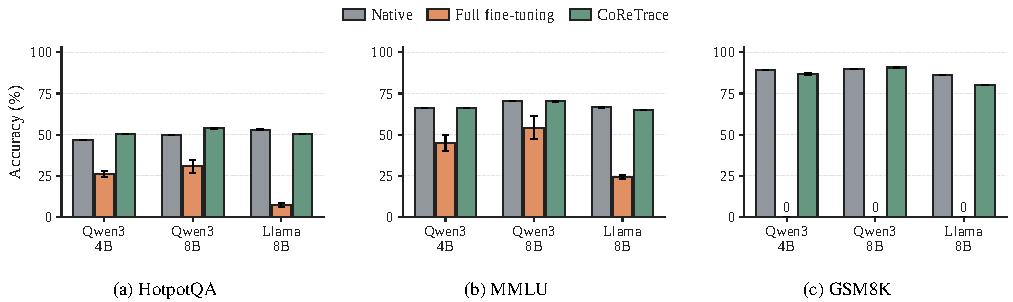
\includegraphics[width=\textwidth]{figures/data_app_capabilities.pdf}
  \caption{\textbf{General capabilities across adaptation methods.} Columns show models and rows show the three complete benchmark splits. Bars report absolute accuracy, with recorded-run SD; annotations give \method's percentage-point change from Native. Fixed restoration recovers 31.92 points on Llama GSM8K over head tuning, and the complete repair improves Qwen HotpotQA over Native. Full fine-tuning's GSM8K score accompanies zero valid final-answer lines.}
  \label{fig:capability_detail}
\end{figure}

\subsection{Answer Quality and Output-Format Adaptation}

\paragraph{Evidence-based answer quality.} The text metrics in \cref{tab:secondary_qa} extend the exact-match results. Qwen3-4B and Qwen3-8B HotpotQA F1 rise from 60.16/63.29\% to 65.13/67.98\%. For Llama, the complete repair raises head-tuning F1 from 56.87\% to 64.31\%, alongside the 7.19-point exact-match recovery. HotpotQA completion reaches 99.93/99.93/99.97\% across the three final models.

\paragraph{Mathematical answer formatting.} Fixed restoration raises Llama's valid GSM8K final-answer rate from 58.61\% under head tuning to 96.36\%, accompanying the increase in numerical accuracy from 48.45\% to 80.36\%. Qwen3-8B improves valid answer formatting from native 95.98\% to 96.82\% and completion from 98.79\% to 99.39\%. The complete format and EOS metrics appear alongside the QA text metrics in \cref{tab:secondary_qa}.

\begin{table}[H]
  \centering
  \caption{\textbf{Secondary answer-quality and completion metrics.} HotpotQA uses its 7,405-example validation split; GSM8K uses its 1,319-example test split. HotpotQA text EM and F1 use accepted normalized aliases, and completion records EOS within the generation budget. GSM8K valid format requires a parsable final \texttt{\#\#\#\# NUMBER} line. Values are percentages averaged across three recorded runs; Native is measured once.}
  \label{tab:secondary_qa}
  \small\setlength{\tabcolsep}{4pt}
  % Generated by analysis/build_tables.py.
\begingroup\renewcommand{\arraystretch}{1.08}
\begin{tabular}{llrrrrr}
\toprule
 &  & \multicolumn{3}{c}{\textbf{HotpotQA}} & \multicolumn{2}{c}{\textbf{GSM8K}} \\
\cmidrule(lr){3-5}\cmidrule(lr){6-7}
\textbf{Model} & \textbf{Method} & \textbf{Text EM} & \textbf{Text F1} & \textbf{Completion} & \textbf{Valid format} & \textbf{Completion} \\
\midrule
\rowcolor{tablebase}Qwen3-4B & Native & $46.94$ & $60.16$ & $98.47$ & $\mathbf{97.19}$ & $99.24$ \\
 & Full fine-tuning & $26.06$ & $38.17$ & $\mathbf{99.99}$ & $0.00$ & $\mathbf{100.00}$ \\
\rowcolor{tableours} & \method\ (Ours) & $\mathbf{50.45}$ & $\mathbf{65.13}$ & $99.93$ & $95.65$ & $99.44$ \\
\midrule
\rowcolor{tablebase}Qwen3-8B & Native & $49.93$ & $63.29$ & $99.07$ & $95.98$ & $98.79$ \\
 & Full fine-tuning & $30.79$ & $43.20$ & $\mathbf{99.95}$ & $0.00$ & $\mathbf{99.97}$ \\
\rowcolor{tableours} & \method\ (Ours) & $\mathbf{53.81}$ & $\mathbf{67.98}$ & $99.93$ & $\mathbf{96.82}$ & $99.39$ \\
\midrule
\rowcolor{tablebase}Llama-3.1-8B & Native & $\mathbf{53.14}$ & $\mathbf{66.91}$ & $99.54$ & $\mathbf{97.95}$ & $98.26$ \\
 & Full fine-tuning & $7.14$ & $11.93$ & $99.45$ & $0.00$ & $\mathbf{99.92}$ \\
\rowcolor{tableours} & \method\ (Ours) & $50.56$ & $64.31$ & $\mathbf{99.97}$ & $96.36$ & $99.55$ \\
\bottomrule
\end{tabular}
\endgroup

\end{table}

\paragraph{Multiple-choice generation.} \Cref{tab:mmlu_generation} reports generated-letter accuracy and formatting on MMLU in addition to the primary option-probability metric. Generated-letter accuracy increases from 7.92/67.06/54.54\% natively to 33.91/69.78/65.11\% under \method. The corresponding valid-format rates rise from 12.58/95.61/84.14\% to 51.27/99.44/99.99\%. These changes show improved adherence to the requested answer format. Subject-macro generated-letter accuracy rises from 9.04/69.55/55.20\% to 37.30/72.49/65.66\%; the complete table also reports macro option-probability accuracy. Head tuning achieves the highest Qwen3-4B generated-letter accuracy at 42.24\%, while the full repair leads the adapted variants for Qwen3-8B and Llama at 69.78\% and 65.11\%.

\begin{table}[H]
  \centering
  \caption{\textbf{MMLU generation and subject-macro diagnostics.} Results on all 14,042 test questions. Generated-letter accuracy evaluates the emitted A/B/C/D answer; valid format requires an accepted option-only response followed by EOS. Macro metrics average over subjects. Option-macro accuracy uses the same first-token option probabilities as the primary micro metric in \cref{tab:retention}. All values are percentages, averaged across recorded runs; Native is measured once.}
  \label{tab:mmlu_generation}
  \small\setlength{\tabcolsep}{4pt}
  % Generated by analysis/build_tables.py.
\begingroup\renewcommand{\arraystretch}{1.08}
\begin{tabular}{llrrrrr}
\toprule
 &  & \multicolumn{2}{c}{\textbf{Generated-letter accuracy}} & \multicolumn{2}{c}{\textbf{Response quality}} & \textbf{Option scores} \\
\cmidrule(lr){3-4}\cmidrule(lr){5-6}\cmidrule(lr){7-7}
\textbf{Model} & \textbf{Method} & \textbf{Micro} & \textbf{Macro} & \textbf{Valid format} & \textbf{Completion} & \textbf{Macro accuracy} \\
\midrule
\rowcolor{tablebase}Qwen3-4B & Native & $7.92$ & $9.04$ & $12.58$ & $97.91$ & $\mathbf{68.38}$ \\
 & Full fine-tuning & $18.26$ & $17.92$ & $34.44$ & $\mathbf{100.00}$ & $46.77$ \\
 & Head tuning & $\mathbf{42.24}$ & $\mathbf{45.66}$ & $\mathbf{63.30}$ & $99.74$ & $68.19$ \\
\rowcolor{tableours} & \method\ (Ours) & $33.91$ & $37.30$ & $51.27$ & $99.52$ & $68.19$ \\
\midrule
\rowcolor{tablebase}Qwen3-8B & Native & $67.06$ & $69.55$ & $95.61$ & $99.97$ & $\mathbf{73.04}$ \\
 & Full fine-tuning & $18.29$ & $18.42$ & $32.05$ & $99.82$ & $56.56$ \\
 & Head tuning & $69.75$ & $72.47$ & $99.44$ & $\mathbf{100.00}$ & $72.93$ \\
\rowcolor{tableours} & \method\ (Ours) & $\mathbf{69.78}$ & $\mathbf{72.49}$ & $\mathbf{99.44}$ & $\mathbf{100.00}$ & $72.92$ \\
\midrule
\rowcolor{tablebase}Llama-3.1-8B & Native & $54.54$ & $55.20$ & $84.14$ & $\mathbf{100.00}$ & $\mathbf{66.77}$ \\
 & Full fine-tuning & $1.06$ & $1.06$ & $4.35$ & $99.62$ & $24.15$ \\
 & Head tuning & $64.36$ & $64.77$ & $99.84$ & $\mathbf{100.00}$ & $64.87$ \\
\rowcolor{tableours} & \method\ (Ours) & $\mathbf{65.11}$ & $\mathbf{65.66}$ & $\mathbf{99.99}$ & $\mathbf{100.00}$ & $65.66$ \\
\bottomrule
\end{tabular}
\endgroup

\end{table}

\subsection{Worked Evidence Chains}

The teaser uses a Llama example whose evidence states that Walter II of Avesnes is the son of James of Avesnes and that James was killed at the Battle of Arsuf. Native constituent answers identify James and Arsuf, whereas the native composed answer is ``Avesnes.'' The final procedure answers ``Arsuf.''

A second example asks who John Corvinus's paternal grandfather was. The supplied chain is John Corvinus $\rightarrow$ Matthias Corvinus $\rightarrow$ John Hunyadi. All three native models answer the two constituent questions correctly but answer the composed question ``Matthias Corvinus.'' All three final models instead answer ``John Hunyadi.'' The input-derived graph has two outgoing candidates, so this example exercises attention-based disambiguation.

\section{Token Use and Observed Execution Cost}
\label{app:efficiency}

\cref{tab:inference_cost} covers all 3,000 triplet queries. Input-token totals exclude separate readout prefills: 190 across all query types, including 103 composed, 85 first-hop, and two second-hop queries. In run 42, composed answer-generation input tokens are 42.5\%, 42.4\%, and 43.7\% of Native. This saves 56.3--57.6\% of input tokens for answer generation. The additional readout workload is concentrated on ambiguous candidates: 10.3\% of composed inputs and 6.3\% of all triplet queries.

\begin{table}[H]
  \centering
  \caption{\textbf{Observed inference workload on all 3,000 triplet queries.} Input tokens are final-generation prompt tokens only; output tokens count generated tokens. Readout prefills are listed separately from final-generation input tokens. Entries summarize recorded runs with the displayed batch sizes under shared-device scheduling.}
  \label{tab:inference_cost}
  \small\setlength{\tabcolsep}{4pt}
  % Generated by analysis/build_tables.py.
\begingroup\renewcommand{\arraystretch}{1.08}
\begin{tabular}{llrrrrr}
\toprule
\textbf{Model} & \textbf{Method} & \textbf{Input tokens (M)} & \textbf{Output tokens (K)} & \textbf{Readout prefills} & \textbf{Batch sizes} & \textbf{Seconds} \\
\midrule
\rowcolor{tablebase}Qwen3-4B & Native & 3.564 & 22.58 & 0 & 1 & 1616 \\
 & Full fine-tuning & 3.564 & 16.39 & 0 & 4 & 905 \\
\rowcolor{tableours} & \method\ (Ours) & 2.238 & 16.43 & 190 & 1/4 & 855 \\
\midrule
\rowcolor{tablebase}Qwen3-8B & Native & 3.564 & 22.18 & 0 & 4 & 906 \\
 & Full fine-tuning & 3.564 & 16.49 & 0 & 4 & 980 \\
\rowcolor{tableours} & \method\ (Ours) & 2.236 & 16.42 & 190 & 4 & 952 \\
\midrule
\rowcolor{tablebase}Llama-3.1-8B & Native & 3.452 & 22.02 & 0 & 1 & 1304 \\
 & Full fine-tuning & 3.452 & 14.89 & 0 & 4 & 984 \\
\rowcolor{tableours} & \method\ (Ours) & 2.194 & 14.70 & 190 & 1/4 & 931 \\
\bottomrule
\end{tabular}
\endgroup

\end{table}
